\chapter{Regular Expression Synthesis}\label{chap:regex-synthesis}

In this chapter, we describe the first stage of \Forest{}'s synthesis procedure, which produces the first component of the regex validation: a regular expression that matches all valid examples and none of the invalid examples. This regular expression serves as basis for the synthesis of the second and third components of the regex validation.


Before the synthesis procedure starts, we define the set of operators that can be used to build the desired regex, as well as the values each operator can take as argument, i.e., \Forest{}'s \ac{DSL}. \Forest{} builds its DSL based on the user-provided examples. Each DSL is dynamically constructed to fit the problem at hand: it is as restricted as possible, without losing any expressiveness necessary to ensure it includes the correct regex. The DSL construction procedure is detailed in \autoref{sec:dsl}.

\begin{figure}[t]
    \centering
    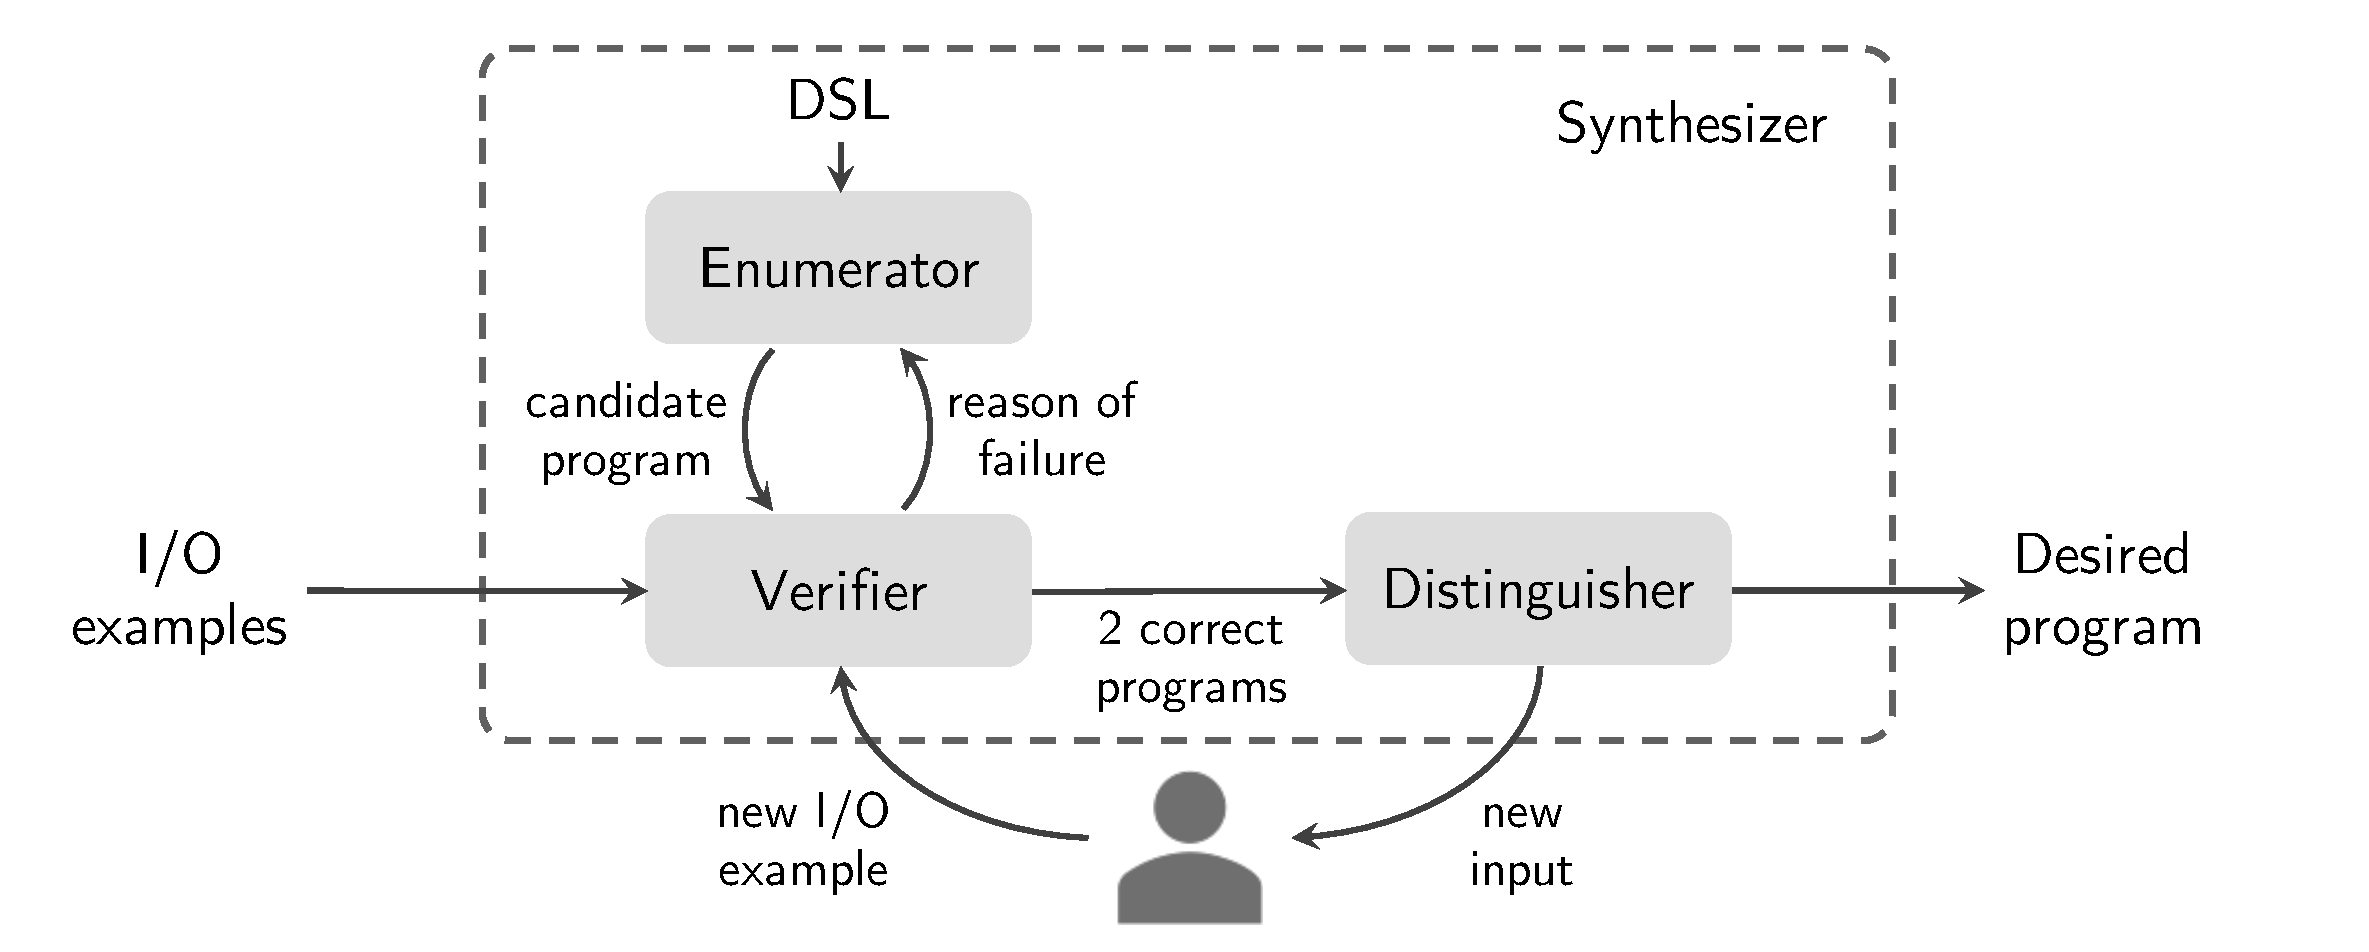
\includegraphics[scale=.35]{pictures/interactive_synthesis.pdf}
    \caption{Interactive enumeration-based synthesis}
    \label{fig:interactive-synthesis}
\end{figure}

Our synthesis algorithm employs enumerative search, as introduced in \autoref{sec:enum-search}. The enumeration cycle finds regexes that are consistent with the user-provided examples. In order to choose an expression among those generated by the enumeration,  \Forest{} interacts with the user. The result of each interaction is a new input-output example that strengthens the original specification. Both the enumeration and the interaction cycles are depicted in \autoref{fig:interactive-synthesis}.

As mentioned before, input-output examples are an ambiguous specification. Thus, \Forest{} does not return the first regex consistent with the examples that it finds, as it may not correspond to the user's intended behaviour. Instead, \Forest{} provides an interaction model. The interactive model is further described in \autoref{sec:regex-interaction}. 


\section{Domain Specific Language}\label{sec:dsl}
Before the synthesis procedure starts, the \ac{DSL} of the enumerated regexes must be defined. This includes the definition of the operators that can be used to build the desired regex, as well as the values each operator can take as~argument. 

\Forest{} aims at producing a regular expression that fully  matches the strings provided as valid examples. We consider a successful match only when the regular expression matches the entire string.
%
To construct the regex, the \ac{DSL} always includes the union %(\verb-|-)
and concatenation operators. As introduced in \autoref{sec:back-regex}, the union of two arbitrary regexes \(r\) and \(s\) creates a new regex, denoted \(r|s\). A string matches \(r|s\) if it matches \(r\) or \(s\). Similarly, the concatenation of any two regexes \(r\) and \(s\), creates a new regex, \(rs\). If a string \(p\) is matched by \(r\) and a string \(q\) is matched by \(s\), then \(pq\) is matched by \(rs\).

In addition, we consider several regular expression quantifiers. A quantifier can be applied to any regex \(r\) and is equivalent to concatenating \(r\) with itself a certain number of times. The \ac{DSL} includes the following quantifiers:
\begin{itemize}
    \item \textit{Kleene} closure (*), which matches 0 or more times,
    \item positive closure (+), which matches 1 or more times,
    \item option (?), which matches 1 or 0 times,
    \item range (\(\{m\}\)), which matches exactly \(m\) times, and
    \item range (\(\{m,n\}\)), which matches at least \(m\) times and at most \(n\) times.
\end{itemize}

\noindent
The possible values for the range operators are limited depending on the valid examples provided by the user. For the single-valued range operator, \(\{m\}\), we consider only the integer values such that \(2 \le m \le l\), where \(l\) is the length of the longest valid example string. Note that \(m = 1\) is not considered since it is the identity function (\(r\)\(\{1\}\) = \(r\)).
In the two-valued range operator, \(\{m,n\}\), the values of \(m\) and \(n\) are limited to integers such that \(0 \le m < n \leq l\), where \(l\) is again the length of the longest valid example string. The tuple (0,1) is not considered, since its semantics are equivalent to that of the option quantifier:~\(r\{0,1\} = r?\).


All operators can be applied to regex literals or composed with each other to form more complex expressions.
The regex literals considered in the synthesis procedure also depend on the valid input examples. These include the individual letters, digits or symbols present in the examples and all character classes that include them.
The character class \texttt{[\(r_1\)-\(r_n\)]} is shorthand for the regular expression  \texttt{\(r_1\)|\(r_2\)|...|\(r_n\)}, when \(r_1 r_2 ... r_n\) form a logical sequence.
The character classes contemplated in the DSL are \texttt{[0-9]}, \texttt{[A-Z]}, \texttt{[a-z]} and all combinations of those, such as \texttt{[A-Za-z]} or \texttt{[0-9A-Za-z]}. Additionally, \texttt{[0-9A-F]} and \texttt{[0-9a-f]} are used to represent hexadecimal numbers.

As mentioned in \autoref{sec:program-space}, the \ac{DSL} can be represented as a \ac{CFG}.
%A \ac{CFG} is defined by a 4-tuple \((N, \Sigma, R, S)\), where \(N\) is a set of non-terminal symbols, \(\Sigma\)~a~set of terminal symbols (disjoint from \(N\)), and \(R\) a set of rules or productions, each of the form \(A \to \beta\), where \(A\) is a non-terminal and \(\beta\) is a string of symbols from the set \((\Sigma \cup N)*\). \(S \in N\) is the designated start symbol.
The \ac{CFG}'s terminal symbols \(\Sigma\) include the names of all regex operators, as well as the regex literals and the range operator values.
\(N\), the non-terminal symbols, are the data~types in the~DSL.

\begin{example}\label{ex:dsl}
The literal values on the DSL depend on the input examples.
Recall the motivating example in \autoref{sec:motivating-example}, where the valid input values were:

\begin{multicols}{3}
    \begin{itemize}[label={}]
    \item 19/08/1996
    \item 26/10/1998
    \item 22/09/2000
    \item 01/12/2001
    \item 29/09/2003
    \item 31/08/2015
    \end{itemize}
\end{multicols}

\noindent
In this scenario, the length of the longest valid example is \(l = 10\), so the range value literals are \(m \in \{2, ..., 10\}\), for the single valued range, and \((n, m): 0 \leq n < m \leq 10\) for the two-valued range. The characters in the examples are `/', which becomes itself a regex literal, and digits, which introduce the character class \texttt{[0-9]}. The \ac{CFG} is then defined as shown in \autoref{fig:dsl}.
%
\end{example}

\begin{figure}[t]
  \begin{align*}
    Re \;\to \;\;&  \Concat(Re, Re) \;\;|\;\;  \Union(Re, Re)   \;\;|\;\;  \Kleene(Re) \;\;|\;\;  \Posit(Re) \\[1.1ex]
          |\;\;&  \Option(Re) \;\;|\;\;  \Range(Re, \Rangelit) \;\;|\;\; \texttt{[0-9]} \;\;|\;\; \texttt{/}\\[1.3ex]
    \Rangelit \;\to \;\;&  2 \;|\; 3 \;|\; ... \;|\; 10 \;|\; (0,2) \,|\, (1,2)\,|\, (0,3) \,|\, ... \,|\, (8,10)\,|\, (9,10)
  \end{align*}
  \captionsetup{belowskip=-7pt, aboveskip=-5pt}
  \caption{\ac{CFG} that represents the \ac{DSL} of regular expressions for the motivating example in \autoref{sec:motivating-example}. \(Re\) is the start symbol and the representation of the regex type, \(\Rangelit{}\) represents the possible values for the argument of the range operator.}
  \label{fig:dsl}
\end{figure}



\section{Enumeration}\label{sec:regex-enumeration}

To enumerate regexes, \Forest{} requires a structure capable of representing every feasible expression. % There are different approaches to achieve this. 
Orvalho et. al. \cite{Orvalho19} describe two different representations: tree-based and line-based. The tree-based representation follows a typical hierarchical composition of operations, as usually seen in functional languages, while the line-based representation emulates the structure of a program written in an imperative language, where each operation is seen as a line of code.

We opt to use a tree-based representation of the search space, using \(k\)-trees. A \(k\)-tree of depth \(d\) is a tree in which every internal node has exactly \(k\) children and every leaf node is at depth \(d\).
If \(k\) is the greatest arity among all DSL constructs, then a \(k\)-tree of depth \(d\) can represent all programs of depth up to \(d\) in that \ac{DSL}. For that, a symbol of the DSL is assigned to each node and the tree can be interpreted as a program. In any regex DSL built by \Forest{}, the maximum arity is always 2, so all regexes in the search space can be represented using 2-trees. In \autoref{fig:date-ktree}, the regex from the motivating example in \autoref{sec:motivating-example}, \UseVerb{date2}, is represented as a 2-tree of depth 5.

To explore the search space in order of increasing complexity, the \(k\)-tree enumerator starts by analysing trees of lower depths and progressively increases the depth of the tree as trees of previous depths are exhausted.
This way we ensure the first regex found is of the smallest depth possible.


\begin{figure}[t]
\centering
\begin{tikzpicture}[
level distance=1.1cm,
level 1/.style={sibling distance=6cm},
level 2/.style={sibling distance=3.6cm},
level 3/.style={sibling distance=1.7cm},
level 4/.style={sibling distance=1.1cm,level distance=.9cm}]
\tikzstyle{every node}=[circle,draw,minimum size=1.4pt]
\tikzstyle{every label}=[rectangle, draw=none]

\node (Root) [label={concat}] {}
child {
    node [label={concat}] {} 
    child {
        node [label={concat}] {} 
        child {
            node [label={range}] {} 
            child { node [label=below:{\Verb![0-9]!}] {} }
            child { node [label=below:{2}] {} }
        }
        child {
            node [label={\texttt{/}}] {} 
            child { node [label={[text=eps-node-color]below:\(\epsilon\)}, draw=eps-node-color, right=.08cm] {} edge from parent[draw=eps-node-color] }
            child { node [label={[text=eps-node-color]below:\(\epsilon\)}, draw=eps-node-color, left=.08cm] {} edge from parent[draw=eps-node-color] }
        }
    }
    child {
        node [label={concat}] {} 
        child {
            node [label={range}] {} 
            child { node [label=below:{\Verb![0-9]!}] {} }
            child { node [label=below:{2}] {} }
        }
        child {
            node [label={\texttt{/}}] {} 
            child { node [label={[text=eps-node-color]below:\(\epsilon\)}, draw=eps-node-color, right=.08cm] {} edge from parent[draw=eps-node-color] }
            child { node [label={[text=eps-node-color]below:\(\epsilon\)}, draw=eps-node-color, left=.08cm] {} edge from parent[draw=eps-node-color] }
        }
    }
}
%
child {
    node [label={range}] {} 
    child {
        node [label={\Verb![0-9]!}, right=.3cm] {}
        child {
            node [label={[text=eps-node-color]:\(\epsilon\)}, draw=eps-node-color, right=0cm] {} edge from parent[draw=eps-node-color]
            child { node [label={[text=eps-node-color]below:\(\epsilon\)}, draw=eps-node-color, right=.08cm] {} edge from parent[draw=eps-node-color] }
            child { node [label={[text=eps-node-color]below:\(\epsilon\)}, draw=eps-node-color, left=.08cm] {} edge from parent[draw=eps-node-color] }
        }
        child {
            node [label={[text=eps-node-color]:\(\epsilon\)}, draw=eps-node-color, left=0cm] {} edge from parent[draw=eps-node-color]
            child { node [label={[text=eps-node-color]below:\(\epsilon\)}, draw=eps-node-color, right=.08cm] {} edge from parent[draw=eps-node-color] }
            child { node [label={[text=eps-node-color]below:\(\epsilon\)}, draw=eps-node-color, left=.08cm] {} edge from parent[draw=eps-node-color] }
        }
    }
    child {
        node [label={4}, left=.3cm] {}
        child {
            node [label={[text=eps-node-color]:\(\epsilon\)}, draw=eps-node-color, right=0cm] {} edge from parent[draw=eps-node-color]
            child { node [label={[text=eps-node-color]below:\(\epsilon\)}, draw=eps-node-color, right=.08cm] {} edge from parent[draw=eps-node-color] }
            child { node [label={[text=eps-node-color]below:\(\epsilon\)}, draw=eps-node-color, left=.08cm] {} edge from parent[draw=eps-node-color] }
        }
        child {
            node [label={[text=eps-node-color]:\(\epsilon\)}, draw=eps-node-color, left=0cm] {} edge from parent[draw=eps-node-color]
            child { node [label={[text=eps-node-color]below:\(\epsilon\)}, draw=eps-node-color, right=.08cm] {} edge from parent[draw=eps-node-color]}
            child { node [label={[text=eps-node-color]below:\(\epsilon\)}, draw=eps-node-color, left=.08cm] {} edge from parent[draw=eps-node-color]}
        }
    }
};

\end{tikzpicture}
\caption{\UseVerb{date2} represented as a \(k\)-tree.}
\label{fig:date-ktree}
\end{figure}{}


To explore the space of trees, the enumerator encodes the \(k\)-tree as an \ac{SMT} formula. 
%
The constraints in the \ac{SMT} formula ensure that the program is well-typed. 
%
A model that satisfies the formula represents an assignment of a DSL symbol to each tree node. This assignment is then used to build a valid regex.

\subsection{\textit{K}-tree Encoding}\label{sec:k-tree}

In this section we offer a formal description of the \(k\)-tree encoding, as proposed by Chen et. al. \cite{DBLP:conf/sigsoft/ChenMF19,Orvalho19}.
Consider a \(k\)-tree of depth \(d\). Assume each node in the \(k\)-tree is assigned a unique positive integer index consistent with level-order traversal. Let \(N\) be the set all nodes' indices, \(N = \{1, 2, ..., k^d - 1\}\).
%
Let \(L\) be the set of indices that correspond to leaf nodes and \(I\) the set of indices of internal nodes. Thus \(N = I \cup L\). Furthermore, let \(C(i)\) represent the indices of all children of node \(i\).

Let \(id: \Sigma \to \mathbb{N}\) be a one-to-one mapping of each terminal symbol (i.e., operators and literals) in the DSL to a positive integer.
Because the arity of some DSL operations is smaller than \(k\), there are some children nodes that cannot be assigned any symbol. We introduce the empty symbol, \(\epsilon\), with \(id(\epsilon) = 0\), which is assigned to nodes without symbols.

\paragraph{Encoding variables.}
We define an integer variable \(n_i\) for all \(i \in N\). Assigning \(n_i = id(k)\) means
that we assign the symbol~\(k\) to node \(i\).

\medskip

Next, we add constraints over these variables that ensure the generated regular expression is well-typed. 
All examples in the remainder of this section refer to the DSL presented in \autoref{ex:dsl} built for the
the motivating example described in \autoref{sec:motivating-example}.

\paragraph{Leaf constraints.} 
Because they have no children, the leaf nodes must be empty or assigned to a literal of the DSL.
Let \(T\) be the union of \(\epsilon\) with the set of terminal symbols in the DSL that correspond to literals.

\begin{equation}
    \bigwedge_{i \in L} \; \bigvee_{p \in T} n_i = id(p)
\end{equation}

\begin{example}\label{ex:leaf-constraints}
For each leaf node \(i\) we add the constraint:
\begin{gather*}
    n_i = id(\texttt{[0-9]}) \lor n_i = id(\texttt{/}) \lor n_i = id(2) \lor ... \lor n_i = id(10) \lor n_i = id((0,2)) \;\lor \\
    \lor\; n_i = id((1,2)) \lor  n_i = id((0,3)) \lor ... \lor  n_i = id((8,10))\lor  n_i = id((9,10)) 
\end{gather*}
\end{example}


\paragraph{Children constraints.}
If a DSL symbol \(p\) is assigned to a node \(i\), the children of \(i\), \(C(i)\), must have types consistent with the parameters of \(p\).
For each \(p \in \Sigma\) and \(j \in \{1, ..., k\}\), where \(k\) is the largest arity among all DSL constructs, we define \(T(p, j)\).
If \(p\) corresponds to an operator, \(T(p, j)\) denotes the type of parameter \(j\) of \(p\). If \({j > arity(p)}\), then \(T(p,j) = \epsilon\).
If \(p\) represents a literal, then \(T(p,j) = \epsilon\) for every~\(j\).
Finally, let \(\Sigma(T(p,j)) \subset \Sigma\) be the set of terminal symbols in the \ac{DSL} that have type \(T(p,j)\).

\begin{equation}
    \bigwedge_{p \in \Sigma, i \in I}\; \left(n_i = id(p) \Rightarrow \bigwedge_{j \in C(i)} \; \bigvee_{t \in \Sigma(T(p,j))} n_j = id(t) \right)
\end{equation}

\begin{example}\label{ex:children-constraints}
If node 1 is assigned \(\Range\), then its children, nodes 2 and 3, must be assigned symbols of types consistent with its parameters. \({T(\Range, 1) = Re}\), so \(n_2\) must be assigned one of the symbols in
\(\Sigma(Re)=\{\Union, \Concat,\allowbreak \Kleene,\allowbreak \Posit,\allowbreak \Option,\allowbreak \Range, \texttt{[0-9]}, \texttt{/}\}\).
\(T(\Range, 2) = \Rangelit\), so \(n_3\) must be assigned one of the symbols in \(\Sigma(\Rangelit) = \{2,\allowbreak ...,\allowbreak 10,\allowbreak (0,2),\allowbreak (1,2),\allowbreak ... ,\allowbreak (9,10)\}\).
To enforce this, we add the following constraint:
\begin{align*}
    n_1=id(\Range) \Rightarrow (&n_2=id(\Union) \lor n_2=id(\Concat) \lor n_2=id(\Kleene) \,\lor\\
    &\lor n_2=id(\Posit) \lor n_2=id(\Option) \lor n_2=id(\Range) \,\lor\\
    &\lor n_2=id(\texttt{[0-9]}) \lor n_2=id(\texttt{/})\,) \\
    \land \, (&n_3=id(2) \lor ... \lor n_3=id(10) \lor n_3=id((0,2)) \,\lor \\
    &\lor\, n_3=id((1,2)) \lor ... \lor  n_3=id((9,10))\,)
\end{align*}
\end{example}

\paragraph{Output constraints.}  
The root node must be assigned a DSL symbol consistent with the output type. \(Re\) is the desired output type in our DSL. Then \(\Sigma(Re)\) is the set of symbols in the DSL that have type \(Re\).

\begin{equation}
    \bigvee_{p\in \Sigma(Re)} n_1 = id(p)
\end{equation}


\begin{example}
We want or regular expression to have the DSL type \(Re\), so the output constraint for our domain is
\begin{gather*}
    n_1 = id(\Union) \lor n_1 = id(\Concat) \lor n_1 = id(\Kleene) \lor n_1 = id(\Posit) \;\lor \\
    \lor\; n_1 = id(\Option) \lor n_1 = id(\Range) \lor n_1 = id(\texttt{[0-9]}) \lor n_1 = id(\texttt{/})
\end{gather*}
\end{example}

\subsection{Multi-tree Representation}\label{sec:multi-tree}
We considered several validators for digital forms and observed that many regexes in this domain are the concatenation of relatively simple regexes. However, the successive concatenation of simple regexes quickly becomes complex in its \(k\)-tree representation.
%
Recall the regex for date validation presented in the motivating example in \autoref{sec:motivating-example}: \UseVerb{date2}.
%
Even though this regular expression is the concatenation of 5 simple sub-expressions, each of which can be represented using a tree of depth at most~2, its representation as a {\(k\)-tree} requires a tree of depth~5, as shown in \autoref{fig:date-ktree}.

\begin{figure}[t]
\centering
\definecolor{top-node-color}{HTML}{3e5561}
\begin{tikzpicture}[
level 1/.style={sibling distance=2cm},
level 2/.style={sibling distance=1cm},
level 1/.append style={level distance=1.5cm},
level 2/.append style={level distance=.8cm},
empty/.style={edge from parent/.style={solid,eps-node-color,draw}}]
\tikzstyle{every node}=[circle,draw=black, solid, edge from parent/.style={solid,eps-node-color,draw=black}]
\tikzstyle{edge from parent}=[draw=black, solid]
\tikzstyle{every label}=[rectangle, draw=none]

\node (Root) [label={[text=top-node-color]:concat}, draw=top-node-color,thick, dotted] {} 
child {
    node [label={range}] {} edge from parent[draw=top-node-color,dashed]
    child {
        node [label=below:{\Verb![0-9]!}, draw=black] {} }
    child {
        node [label=below:{2}] {} }
}
%
child {
    node [label={\texttt{/}}] {} edge from parent[draw=top-node-color,dashed]
    child[empty] {
        node [label={[text=eps-node-color]below:\(\epsilon\)}, draw=eps-node-color] {}}
    child[empty] {
        node [label={[text=eps-node-color]below:\(\epsilon\)}, draw=eps-node-color] {}}
}
%
child {
    node [label={range}] {} edge from parent[draw=top-node-color,dashed]
    child {
        node [label=below:{\Verb![0-9]!}] {} }
    child {
        node [label=below:{2}] {} }
}
%
child {
    node [label={\texttt{/}}] {} edge from parent[draw=top-node-color,dashed]
    child {
        node [label={[text=eps-node-color]below:\(\epsilon\)}, draw=eps-node-color] {}  edge from parent[draw=eps-node-color] }
    child {
        node [label={[text=eps-node-color]below:\(\epsilon\)}, draw=eps-node-color] {}  edge from parent[draw=eps-node-color] }
}
%
child {
    node [label={range}] {}edge from parent[draw=top-node-color,dashed]
    child {
        node [label=below:{\Verb![0-9]!}] {} }
    child {
        node [label=below:{4}] {} }
};

\end{tikzpicture}
\caption{\UseVerb{date2} represented as a multi-tree, resulting from the concatenation of 5 simpler regexes.}
\label{fig:date-multitree}
\end{figure}{}

The idea behind the multi-tree constructs is to allow the number of concatenated sub-expressions to grow without it reflecting exponentially on the encoding. The multi-tree structure is constituted by \(n\) \(k\)-trees, whose roots are connected by an artificial top-level root node. The root-node is ``assigned'' an \(n\)-ary concatenation operator, whose semantics is analogous to that of the binary concatenation of regexes described in \autoref{sec:dsl}. Since the return type of \Concat{} is the same as that of its parameters, \(Re\), all the root nodes have the same type as they did in the original \(k\)-tree encoding. % Thus, each of the \(n\) trees is encoded with \(k\)-tree encoding. 
Because the root-node has a fixed assignment, it is not included in the \ac{SMT} encoding, and it is artificially added to the model that satisfies it.

Having a top-level concatenation node that connects \(n\) \(k\)-trees of depth \(d\), we are able to represent regexes using fewer nodes. \autoref{fig:date-multitree} shows the multi-tree representation of the same regex as \autoref{fig:date-ktree}, and shows that the multi-tree construct can represent this expression using half the~nodes.

In the \(k\)-tree encoding, an increase in the depth \(d\) of the tree corresponds to an increase in the expression's complexity. Thus, the enumerator successively explores \(k\)-trees of increasing depth. However, multi-tree has 2 measures of complexity: the depth of the trees, \(d\), and the number of trees, \(n\). Note that, since it is not encoded into \ac{SMT}, the root-node level is not taken into account for the depth of the multi-tree. \Forest{} employs two different methods for increasing these values: static multi-tree and dynamic multi-tree.


\subsubsection{Static multi-tree} \label{sec:static-multi-tree} In the static multi-tree method, \Forest{} fixes \(n\) and progressively increases \(d\). To find the value of \(n\), there is a preprocessing step, in which \Forest{} identifies patterns in the valid examples. This is done by first identifying substrings common to all examples. A substring is considered a dividing substring if it occurs exactly the same number of times in all examples. Dividing substrings must also occur in the same order in all examples. Then, we split each example before and after the dividing substrings. Each example becomes an array of \(n\) strings.

\begin{example}\label{ex:splitting}
Consider the valid examples from the motivating example in \autoref{sec:motivating-example}.
%
In these examples, `/' is a dividing substring because it occurs in every example, and exactly twice in each one. `0' is a common substring but not a dividing substring because it does not occur the same number or times in all examples. After splitting on `/', each example becomes a tuple of 5 strings:

\begin{multicols}{3}
    \begin{itemize}[label={}]
    \item (`19', `/', `08', `/', `1996')
    \item (`26', `/', `10', `/', `1998')
    \item (`22', `/', `09', `/', `2000')
    \item (`01', `/', `12', `/', `2001')
    \item (`29', `/', `09', `/', `2003')
    \item (`31', `/', `08', `/', `2015')
    \end{itemize}
\end{multicols}
\end{example}
%
\noindent
Then, we apply the multi-tree method with \(n\) trees. If, for every \(i \in \{1, ..., n\}\), the \(i^{th}\) sub-tree represents a regex that matches all strings in the \(i^{th}\) position of the example arrays, then the concatenation of the \(n\) regexes matches the original example strings.
%
Since each tree is only synthesizing for a part of the original input strings, a reduced DSL can be recomputed for each~tree. %Each tree's DSL is contained in the original DSL.

\begin{example}
Recall the split examples from \autoref{ex:splitting}, and the DSL built before the split shown in \autoref{fig:dsl}. This DSL has two regex literals, \texttt{/} and \texttt{[0-9]}. However, we can see that only \texttt{[0-9]} is needed in the \nth{1}, \nth{3} and \nth{5} splits. Moreover, since the length of the splits is smaller than 10, fewer values for \(\Rangelit\) need to be considered.
We can build 5 reduced DSLs, \(\{D_1, D_2, D_3, D_4, D_5\}\), where each \(D_i\) includes only the required symbols to build the regex that matches the \(i^{th}\) split. \(D_1 = D_3\) are represented~as:
\begin{align*}
Re \;\to \;\; &\Concat(Re, Re) \;\;|\;\;  \Union(Re, Re)   \;\;|\;\;  \Kleene(Re) \;\;|\;\; \Posit(Re)\\
     |\;\;    &\Option(Re) \;\;|\;\;  \Range(Re, \Rangelit) \;\;|\;\; \texttt{[0-9]}\\
%
\Rangelit \;\to \;\;& 2 \;|\; (0,2) \,|\, (1,2)
\end{align*}
%
Analogously, \texttt{[0-9]} is never needed in the \nth{2} and \nth{4} splits. \(D_2 = D_4\) are represented as:
%
\begin{align*}
Re \;\to \;\; &\Concat(Re, Re) \;\;|\;\;  \Union(Re, Re)   \;\;|\;\;  \Kleene(Re) \\
        |\;\; &\Posit(Re) \;\;|\;\; \Option(Re) \;\;|\;\; \texttt{/}
\end{align*}
In the \nth{2} and \nth{4} splits, the maximum length is 1, which means there are no possible values for the range operator. Thus, \(\Range\) is not part of \(D_2\) and \(D_4\).
\(D_5\) is similar to \(D_1\) and \(D_3\) but it has more possible values for \Range{}, since the maximum length is 4.
Now, each of the 5 \(k\)-trees can use the corresponding \(D_i\) instead of the whole original DSL.
\end{example}

\subsubsection{Dynamic multi-tree}\label{sec:dynamic-multi-tree} The dynamic multi-tree method is employed when the examples cannot be split because there are no dividing substrings.
In this scenario, the enumerator still uses a multi-tree construct to represent the regex. However, the number of trees is not fixed and all trees use the original, complete DSL. 
\Forest{} varies the complexity of the enumerated expressions by increasing either the number of trees \(n\) or their depth \(d\).
A multi-tree structure with \(n\) \(k\)-trees of depth \(d\) has \(n \times (k^d - 1)\) nodes.
Different combinations of \((n, d)\) are tested in increasing order of number of nodes, starting with \(n = 1\) and \(d = 2\), which is equivalent to a simple \(k\)-tree of depth 2.
\begin{comment}
The pairs \((n, d)\) tested in the first 10 iterations of the dynamic multi-tree enumeration are shown in \autoref{tab:dynamic-mt-growth}.
\begin{table}[t]
\centering
\setlength{\tabcolsep}{2ex} \renewcommand{\arraystretch}{1.2}
\begin{tabular}{@{}cccc@{}}

\toprule
iteration & \(d\) & \(n\) & \# nodes \\ \midrule
1         & 2     & 1     & 3  \\
2         & 2     & 2     & 6  \\
3         & 3     & 1     & 7  \\
4         & 2     & 3     & 9  \\
5         & 2     & 4     & 12 \\
6         & 3     & 2     & 14 \\
7         & 2     & 5     & 15 \\
8         & 4     & 1     & 15 \\
9         & 2     & 6     & 18 \\
10        & 2     & 7     & 21 \\
...       & ...   & ...   & ...      \\\bottomrule
\end{tabular}
\caption{Values of \(n\) and \(d\) for each iteration of dynamic multi-tree enumeration.}
\label{tab:dynamic-mt-growth}
\end{table}
\end{comment}


\subsection{Pruning}\label{sec:pruning}
The tree-based representation is especially advantageous when pruning the search space, as it facilitates the propagation of constraints from any node in the tree to the leaves.
\Forest{} applies two kinds of pruning techniques. The first kind refer to properties of the DSL that remain unchanged during the synthesis procedure and are added at the beginning, along with the encoding~constraints. %The second kind refer to characteristics of the current instance and are added during enumeration.

Like in most other languages, there can be multiple regexes that, although different, have the same semantics. Here are some examples of such equivalences:
%
\begin{comment}
\begin{multicols}{2}
\begin{enumerate}
  \item \((r*)* = r*\)
  \item \((r?)? = r?\)
  \item \((r+)+ = r+\)
  \item \((r+)* = (r*)+ = r*\)
  \item \((r?)* = (r*)? = r*\)
  \item \((r?)+ = (r+)? = r*\)
  \item \((r*)\{m\} = (r\{m\})*\)
  \item \((r+)\{m\} = (r\{m\})+\)
  \item \((r?)\{m\} = (r\{m\})?\)
  \item \(r\{n\}\{m\} = r\{m\}\{n\} = r\{m\times n\}\)
\end{enumerate}
\end{multicols}
\end{comment}
%
\begin{align*}
 (r*)* &\equiv r*               &  (r?)? &\equiv r?             &  (r+)+ &\equiv r+ \\
 (r+)* \equiv\;&(r*)+ \equiv r*       &  (r?)* \equiv\;&(r*)? \equiv r*     &  (r?)+ \equiv(&r+)? \equiv r* \\
 (r*)\{m\} &\equiv (r\{m\})*    & (r+)\{m\} &\equiv (r\{m\})+   & (r?)\{m\} \equiv&\; (r\{m\})? \\
                  &&r\{n\}\{m\} \equiv r\{m\}&\{n\} \equiv r\{m\times n\}&&
\end{align*}
\noindent
During the synthesis procedure, we want to avoid enumerating several equivalent expressions. To achieve this, we add \ac{SMT} constraints that block all but one possible representation of each regex. Take, for example, \({(r?)+ \equiv r*}\). We only want one way to represent this regex, so we block the construction \((r?)+\) for any regex \(r\).
%In the tree-based structure, this is equivalent to saying that if a node is assigned \Option{}, its parent should not be assigned \Posit{}.
Let \(I\) be the set of indices of all internal nodes of the trees and \(Ch_L(i)\) denote the index of the left child of node~\(i\). We add the~constraint:
% Then, to prevent the enumeration of any regex of the form \(r?^+\), we add the constraint:
\begin{equation}
     \bigwedge_{i \in I} n_{Ch_L(i)} = id(\Option{}) \Rightarrow n_i \ne id(\Posit{})
\end{equation}
The remaining equivalences shown above are implemented analogously.

Another relevant rule in the DSL of regular expressions is the idempotence of union: \(r|r = r\).
To prevent the enumeration of expressions of the type \(r|r\), every time the \Union{} operator is assigned to a node \(i\), %its parameters must be different from one another. Since these parameters can be any regex,
we force the sub-tree underneath \(i\)'s left child to be different from the sub-tree underneath \(i\)'s right child by at least one node.
For each internal node \(i \in I\), let \(L_i\) (resp. \(R_i\)) be an ordered list of the indices of all nodes in \(i\)'s left (resp. right) child sub-tree, i.e., the sub-tree whose root is \(i\)'s left (resp. right) child. % and whose leaves correspond to the \(k\)-tree's leaves.
%Let \(R_i\) a similar ordered list of the indices of all nodes in \(i\)'s right child sub-tree.
We add the following constraint to ensure the parameters of \Union{} are different:
\begin{equation}
  \bigwedge_{i \in I} \left( n_i = id(\Union{}) \Rightarrow \bigvee_{1 \le j \le |L_i|} n_{L_i[j]} \ne n_{R_i[j]} \right)
\end{equation}

The second kind of pruning constraints are added during enumeration. These do not refer directly to properties of regexes, but rather to characteristics of the current instance. When a regex that is not consistent with the examples is enumerated, it is eliminated from the search space. 
%This is done by adding one constraint that ensures that at least one node is assigned a different DSL symbol than before.
Let \(m: \mathcal{N} \to \mathbb{N}\) be a model to the formula resulting from the encoding of the trees, i.e., an assignment of each \ac{SMT} variable, \(n_i\), to a DSL symbol's identifier. For each encoding variable \(n_i\), \(m(n_i) = id(p)\) means that $p$ was the DSL symbol assigned to node $i$ in the previous solver call.
%
Thus, %after each unsuccessful solver call, 
we block the current regex by adding the constraint:
\begin{equation}
  \bigvee_{i \in N} n_i \ne m(n_i).
\end{equation}

\noindent
Along with the incorrect regex, we want to eliminate regexes that are equivalent to it. The union operator in the regular expressions DSL is commutative: \(r|s = s|r\), for any regexes \(r\) and \(s\). Thus, whenever an expression containing \(r|s\) is discarded, we eliminate the expression that contains \(s|r\) in its place as well.
%
Let \(U\) contain all the indices of the nodes that were assigned the \Union{} operator in the previous solver call: \(U = \{i \in N: m(n_i) = id(\Union{})\}\). First, we block the assignment of all the nodes in the tree that are not descendant from the \Union{} node. Then, we prevent the variables on \(i\)'s left child sub-tree from being assigned the equivalent model value on the right sub-tree, and vice-versa:
\begin{equation}
\bigwedge_{i \in U} \;\Biggl(\;
\bigvee_{i \in N \setminus (L_i \cup R_i)} n_i \ne m(n_i) \;\lor
\bigvee_{1 \le j \le |L_i|} n_{L_i[j]} \ne m(n_{R_i[j]}) \;\lor
\bigvee_{1 \le k \le |R_i|} n_{R_i[k]} \ne m(n_{L_i[k]}) \Biggr)
\end{equation}

\noindent
Besides expressions that are equivalent to the incorrect enumerated expression, we also remove from the search space other expressions that fail in the same way. The goal of quantifiers \Kleene{}, \Posit{} and \Range{} is to allow a regex to be matched more than once. If \Kleene{} is assigned to the root of one of the \(k\)-trees, this tree represents \(r*\), where \(r\) is an arbitrary regex. We test all valid examples for the presence of \(r\{2\}\). If \(r\{2\}\) is not present in any of the examples, we block the expression \(r*\). The same procedure is followed for \Posit{} and \Range{}.

\subsection{Sketch-based}\label{sec:regex-sketches}

As introduced in \autoref{sec:rel-sketching}, some state-of-the are synthesizers use sketches to speed up their enumerative search. Different methods are used to generate and complete sketches. In this section we describe a few of them, which we implemented in \Forest{}.

\subsubsection{Sketch generation}

When enumerating sketches, the procedure is very similar to the one used to enumerate programs: we have a multi-tree construct and successively enumerate sketches using the \(k\)-tree encoding for each sub-tree. 
The main difference between sketch enumeration and the usual regex enumeration procedure lies in the \ac{DSL}: we adapt the \ac{DSL} to produce incomplete programs (with holes) instead of complete regexes. 
We remove literal values and constants from the \ac{DSL}. We introduce two types of ``hole'' to replace them: the regex-hole \(\square_{\textit{re}}\) and the range-hole \(\square_{\textit{range}}\). Then, each sketch can be completed with concrete regex and range literals to get a complete regular expression.

\begin{figure}[t]
  \begin{align*}
    Re \;\to \;\;&  \Concat(Re, Re) \;\;|\;\;  \Union(Re, Re)   \;\;|\;\;  \Kleene(Re) \;\;|\;\;  \Posit(Re) \\[1.1ex]
          |\;\;&  \Option(Re) \;\;|\;\;  \Range(Re, \square_{\textit{range}}) \;\;|\;\; \square_{\textit{re}}
  \end{align*}
  \caption{\ac{CFG} that represents the sketch \ac{DSL} of regular expressions for the motivating example in \autoref{sec:motivating-example}. }
  \label{fig:sketch-dsl}
\end{figure}

\begin{example}
Recall the DSL built for the motivating example in \autoref{sec:motivating-example} shown in \autoref{fig:dsl}. If we were synthesising this instance with sketch-based enumeration, we would have the DSL shown in \autoref{fig:sketch-dsl}, where the regex literals have been replaced with regex-holes, \(\square_{\textit{re}}\), and the range values with range-holes,~\(\square_{\textit{range}}\).
\end{example}

\noindent
Note that we enumerate fewer sketches than we enumerate programs during the standard enumeration procedure, because each sketch corresponds to many concrete programs. In \autoref{fig:date-sketch-multitree}, we can see the sketch that has to be enumerated during sketch-enumeration in order to synthesise \UseVerb{date2} during sketch-completion.

\definecolor{eps-node-color-1}{HTML}{B0B0B0}
\begin{figure}[t]
\centering
\definecolor{top-node-color}{HTML}{3e5561}
\begin{tikzpicture}[
level 1/.style={sibling distance=2cm},
level 2/.style={sibling distance=1cm},
level 1/.append style={level distance=1.5cm},
level 2/.append style={level distance=.8cm},
empty/.style={edge from parent/.style={solid,eps-node-color-1,draw}}]
\tikzstyle{every node}=[circle,draw=black, solid, edge from parent/.style={solid,eps-node-color-1,draw=black}]
\tikzstyle{edge from parent}=[draw=black, solid]
\tikzstyle{every label}=[rectangle, draw=none]

\node (Root) [label={[text=top-node-color]:concat}, draw=top-node-color,thick, dotted] {} 
child {
    node [label={range}] {} edge from parent[draw=top-node-color,dashed]
    child {
        node [label=below:{\scriptsize\textit{Re}}, draw=black, rectangle] {} }
    child {
        node [label=below:{\scriptsize\textit{Range}}, draw=black, rectangle] {} }
}
%
child {
    node [label=below:{\scriptsize\textit{Re}}, rectangle] {} edge from parent[draw=top-node-color,dashed]
    child[empty] {
        node [label={[text=eps-node-color-1]below:\(\epsilon\)}, draw=eps-node-color-1] {}}
    child[empty] {
        node [label={[text=eps-node-color-1]below:\(\epsilon\)}, draw=eps-node-color-1] {}}
}
%
child {
    node [label={range}] {} edge from parent[draw=top-node-color,dashed]
    child {
        node [label=below:{\scriptsize\textit{Re}}, draw=black, rectangle] {} }
    child {
        node [label=below:{\scriptsize\textit{Range}}, draw=black, rectangle] {} }
}
%
child {
    node [label=below:{\scriptsize\textit{Re}}, rectangle] {} edge from parent[draw=top-node-color,dashed]
    child {
        node [label={[text=eps-node-color-1]below:\(\epsilon\)}, draw=eps-node-color-1] {}  edge from parent[draw=eps-node-color-1] }
    child {
        node [label={[text=eps-node-color-1]below:\(\epsilon\)}, draw=eps-node-color-1] {}  edge from parent[draw=eps-node-color-1] }
}
%
child {
    node [label={range}] {}edge from parent[draw=top-node-color,dashed]
    child {
        node [label=below:{\scriptsize\textit{Re}}, draw=black, rectangle] {} }
    child {
        node [label=below:{\scriptsize\textit{Range}}, draw=black, rectangle] {} }
};

\end{tikzpicture}
\caption{Sketch multi-tree whose completion results in \UseVerb{date2}.}
\label{fig:date-sketch-multitree}
\end{figure}{}

\subsubsection{Sketch completion}

To perform sketch-completion, we need to bring back into consideration the information we removed from the \ac{DSL} during sketch-enumeration, i.e., the possible literal values that can be used to fill each hole in our sketch.

\begin{example}
Consider, once again, the motivating example described in \autoref{sec:motivating-example}. If we are synthesising this instance using sketch-based enumeration, the following domains are considered for each hole in the sketches:
\begin{itemize}
    \item \(\set{D}(\square_{\textit{re}})\) = \{\texttt{[0-9]}, \texttt{/}\}
    \item \(\set{D}(\square_{\textit{range}})\) = \{2, 3, ..., 10, (0,2), (1,2), (0,3) , ..., (8,10), (9,10)\}
\end{itemize}
\end{example}

Several methods can be used to find the correct values to fill the holes in a sketch within the respective domain. In \Forest{}, we tried two different approaches: graph-based and \ac{SMT}-based sketch completion.


\paragraph{Graph-based completion} is implemented as described by \citeauthor{DanielThesis} in his MSc. Thesis \cite{DanielThesis}. We start by identifying all possible complete programs resulting from a sketch. To do this, we first consider the root node and recursively visit all its descendants, traversing the sketch tree in \ac{DFS} order. For each tree node we visit, if it is an internal node, we visit its descendants. If it is a hole, we return a list of all possible completions for it, i.e., the values in its corresponding domain. These values are stored in the parent node. In the end of the traversal, each internal node has a list of all possible completions for all holes in its descendant sub-tree. The root node contains information about all completion values for all holes in the tree. Then, the complete programs resulting from the sketch are simply the Cartesian product of all domains stored in the root node. Each concrete program is built and tested against the specification by the \textit{verifier}, and the synthesizer stores those that satisfy the specification.

\paragraph{SMT-based completion} tries to use logic-based reasoning during the completion.
We do not seek \textit{all} possible completions for a sketch, but rather a set of completions that satisfy our specification.
In a way, we are pulling the \textit{verifier}'s role into the sketch completion procedure.
The implementation of this method requires an \ac{SMT} solver with a regex theory, such as Z3 \cite{z3,z3str317}.
The first step is the same as Graph-based completion: traverse the sketch tree and get the possible domains for each hole.

Ideally, we want to assign to each hole in the sketch an SMT variable of type regex, whose domain is limited according to that hole's domain. Then, we would write the sketch regex in SMT using these variables. Finally, we add constraints that state the desired regex must match all valid examples and none of the invalid. If the formula is unsatisfiable, then the sketch cannot be completed in a way that satisfies the specification, and can be discarded. If the formula is satisfiable, the resulting model results in a completion of the sketch that is consistent with the specification.
However, Z3's regex theory is not sufficiently expressive to allow this method's implementation: there cannot be variables inside an SMT regular expression. Therefore, our SMT-based completion is done as follows:

For each sketch \(S\), let \(\set{S}^*\) be the set of all regexes that result from the completion of \(S\). This set is obtained from the Cartesian product of all holes' domains, as before. For each regex \(r_i \in \set{S}^*\) we define an SMT predicate, \(\rho_i\), such that, for any input string \(s\), \(\rho_i(s)\) is \true if and only if regex \(r_i\) matches \(s\). Let \set{V} be the set of all valid examples and \set{I} the set of all invalid examples. For each \(i \in \{1, ..., |\set{S}^*|\}\), we define a Boolean variable \(m_i\) that is assigned \true if and only if the respective \(r_i\) matches all valid examples, \set{V}, and none of the invalid examples, \set{I}:
\begin{equation}
    \bigwedge_{i \in \{1, ..., |\set{S}^*|\}} m_i \leftrightarrow
    \left( \bigwedge_{x \in \set{V}} \rho_i(x) \land \bigwedge_{x \in \set{I}} \neg \rho_i(x) \right).
\end{equation}

\noindent
We want to find a regex \(r_i\) whose \(m_i\) is \true. Thus, we add the constraint:
\begin{equation}
    \bigvee_{i \in \{1, ..., |\set{S}^*|\}} m_i
\end{equation}

If this formula is unsatisfiable, there is no possible completion of sketch \(S\) that matches the specification. If it is satisfiable, then we store the regexes \(r_i\) whose \(m_i\) are assigned \true in the resulting model. All these are correct regexes.

%\paragraph{Hybrid completion}
%Experimental results: UNSAT sketches: faster in SMT, SAT sketches: faster in graph-based. Solution: hybrid method. Try SMT-based completion with a timeout. If UNSAT, move on to next sketch. If SAT, valid completion. If timeout, run graph-based. \todo{Finish}

\section{User Interaction} \label{sec:regex-interaction}

To solve possible ambiguities in the user-provided input-output examples, we implemented in \Forest{} two different interaction models: conversational clarification, as described in \autoref{sec:rel-conv-clarification} and a variation of Ramos's interaction models, as described in \autoref{sec:rel-ramos-interaction}.

\subsection{Conversational Clarification}\label{sec:interaction-cc}

To increase confidence in \Forest{}'s solution, \Forest{} disambiguates the specification by interacting with the user. % so he or she can provide further information about the intended regex.
We employ the interaction method described by Mayer et. al. \cite{DBLP:conf/uist/MayerSGLMPSZG15}, which has been successfully used in several synthesizers  \cite{DBLP:journals/pvldb/LiCM15,DBLP:conf/sigmod/WangCB17,DBLP:conf/pldi/WangCB17}.
%During the synthesis procedure, \Forest{} presents the user with certain inputs and requests the correct output for it. Then synthesizer then uses the answers to resolve ambiguities in the examples. 
Upon finding two regexes that satisfy the user-provided examples, \(r_1\) and \(r_2\), \Forest{} computes a new input that is matched by one of the regexes but not by the other: a \textit{distinguishing input}.     
To produce a distinguishing input, we use an \ac{SMT} solver with a regex theory, such as Z3 \cite{z3,z3str317}, to create two \ac{SMT} predicates \(\rho_{1}\) and \(\rho_{2}\) such that, for any input string \(s\), \(\rho_{1}(s)\) (resp. \(\rho_{2}(s)\)) evaluates to \true{} if and only if \(r_1\) (resp \(r_2\)) matches \(s\).
Then, we use the \ac{SMT} solver to solve the~formula:
%
\begin{equation}\label{eq:regex_distinguishing}
  \exists s: \rho_{1}(s) \neq \rho_{2}(s).
\end{equation}
%
If (\ref{eq:regex_distinguishing}) is satisfiable, the string \(s\) that satisfies it is a distinguishing input. Once found, \Forest{} asks the user to classify this input as valid or invalid.
The distinguishing input along with its correct output form a new input-output pair which is added to the specification, effectively eliminating either \(r_1\) or \(r_2\) from the search space.
If, on the other hand, (\ref{eq:regex_distinguishing}) is unsatisfiable then \(r_1\) and \(r_2\) are equivalent; \Forest{} keeps the shortest regex and discards the~other.

After the first interaction with the user, the synthesis procedure continues only until the end of the current depth and number of trees. Therefore, if the desired expression requires a larger depth than that of the first enumerated expression that satisfied the examples, then \Forest{} never enumerates the desired expression and the returned expression will not satisfy the user's needs in corner cases not covered by the initial examples.

\begin{example}
Consider, for example, that \Forest{} enumerated two regexes consistent with the examples in the motivating example in \autoref{sec:motivating-example}:
\(r_1\) = \Verb![0-9]{2}/[0-9]{2}/[0-9]{3,4}!
and
\(r_2\) = 
\Verb![0-9]{2}/[0-9]{2}/[0-9]{4}!. 
A possible distinguishing input between \(r_1\) and \(r_2\) returned by \Forest{} is \(s\) = ``00/24/404''. This input would be shown to the user. Since it does not represent a valid date, the user would classify \(s\) as invalid. Thus, ``00/24/404'' would be added to the set of invalid examples, and \(r_1\), which matches \(s\), would be eliminated from the search space.
\end{example}



\subsection{Multi-distinguish}\label{sec:multi-dist}

Besides the basic conversational clarification model, we extend \Forest{} with a new interaction model, based on the interaction models first introduced in \citeyear{UnchartIt20} by \citet{UnchartIt20}. 
As mentioned in \autoref{sec:regex-interaction}, \citeauthor{UnchartIt20} present two interaction models: \ynmodel and \optmodel.
In the domain of regular expressions, the output is a Boolean value: either the string is matched by the regular expression or it is~not. In practice, this entails a simplification of the \ynmodel and \optmodel models, and they converge into a single model, which we call multi-distinguish interaction model.

The goal is to distinguish more than two regular expressions at once. Instead of triggering an interaction cycle right after finding two correct regular expressions, we continue the enumeration process past the second expression, until we have \(n\) correct expressions. Then, we disambiguate those \(n\) expressions at once, in order to generate fewer, more comprehensive distinguishing inputs, thus reducing the number of necessary queries to the user.

To disambiguate \(n\) regular expressions, \(r_1, ..., r_n\), we start, as before, by defining \(n\) \ac{SMT} predicates, \(\rho_1, ..., \rho_n\) such that, for any input string \(s\), \(\rho_i(s)\) evaluates to \true{} if and only if \(r_i\) matches \(s\).
We want to find a distinguishing string \(s\) that separates the regexes in two disjoint sets, \set{A} and \set{B}, such that all regexes in \set{A} match \(s\) and none of the regexes in \set{B} matches \(s\). Ideally, we want \set{A} and \set{B} to have the same number of regexes, so we can eliminate at least half the candidate expressions with each interaction.

To ensure at least two regexes in \(r_1, ..., r_n\) produce a different result when matched against \(s\), we add the hard constraint:
\begin{equation}\label{eq:multi-distinguish0}
    \bigvee_{i,j \in \{1, ..., n\}, i<j} \; \rho_i(s) \ne \rho_j(s).
\end{equation}

\noindent
Then, we want to split the regexes into two sets \set{A} and \set{B} of approximately the same size. This problem can be modelled as a bipartite graph. Let the regexes be the vertices in the graph, and let there be an edge between \(r_i\) and \(r_j\) if and only if \(r_i\) and \(r_j\) have a different matching result to string \(s\). Then the graph's sets are equivalent to to sets \set{A} and \set{B}. The resulting structure is a complete bipartite graph, a bipartite graph where each vertex of the first set is connected to every vertex of the second set.

Now, we want to build a bipartite graph such that both sets of vertices have the same size. Since the number of edges in the bipartite graph is \(|\set{A}| \cdot |\set{B}|\), this is equivalent to maximising the number of edges in the graph, i.e., the number of pairs (\(r_i, r_j\)) which have different matching results to \(s\).

Thus, to encode the goal of \set{A} and \set{B} having the same size, we add the soft constraints:
\begin{equation}\label{eq:multi-distinguish}
    \bigwedge_{i,j \in \{1, ..., n\}, i<j} \; \rho_i(s) \ne \rho_j(s).
\end{equation}

We use a \ac{MaxSMT} solver to find a model to this formula. If  \eqref{eq:multi-distinguish0} is unsatisfiable, then all regexes in \(r_1, ..., r_n\) are equivalent and we can keep only one of them. Otherwise, if the formula is satisfiable, \(s\) is a distinguishing string. Once found, \Forest{} follows a similar procedure to that described in \autoref{sec:interaction-cc}: we ask the user to classify \(s\) as valid or invalid. Then, \Forest{} adds the example to the respective set, eliminating from the search space all regexes which are not in accordance to the user's~answer. 


\begin{example}
Suppose \Forest{} enumerates the following four regular expressions:
\begin{itemize}[label={},nosep]
    \item \(r_1\) = \verb`[0-9]{2}/[0-9]{0,2}/[0-9]{3,4}`,
    \item \(r_2\) = \verb`[0-9]{2}/[0-9]{0,2}/[0-9]{4}`,
    \item \(r_3\) = \verb`[0-9]{2}/[0-9]{2}/[0-9]{4}`, and
    \item \(r_4\) = \verb`[0-9]{2}/[0-9]{2}/[0-9]{3,4}`.
\end{itemize}
%
A possible distinguishing input obtained using multi-distinguish is \(s\) = `01//2000'. \(s\) is accepted by \(r_1\)~and~\(r_2\) but not by \(r_3\)~or~\(r_4\). If we show \(s\) to the user, the user classifies it as invalid because it does not correspond to a valid date. We add this example to the set of invalid examples, thus eliminating \(r_1\)~and~\(r_2\) from the search space.
\end{example}
